% Prof. Dr. Ausberto S. Castro Vera
% UENF - CCT - LCMAT - Curso de Ci\^{e}ncia da Computa\c{c}\~{a}o
% Campos, RJ,  2020
% Disciplina: Paradigmas de Linguagens de Programa\c{c}\~{a}o
% Aluno:



\chapter{ Introdu\c{c}\~{a}o}

Neste documento apresentaremos ....

N\~{a}o esque\c{c}a : entre o t\'{\i}tulo e a primeira se\c{c}\~{a}o do cap\'{\i}tulo deve se incluir algum texto, explicando o que deve conter este cap\'{\i}tulo (as principais se\c{c}\~{o}es).


   \section{Aspectos hist\'{o}ricos da linguagem R}



Algumas linguagens s\~{a}o consideradas  tradicionais (como mostrado na Fig.\ref{ling1}) e outras s\~{a}o consideradas modernas (ver Fig.\ref{ling2}). Devemos observar aqui, que a inclus\~{a}o de qualquer figura, significa que ela deve ser referenciada em algum lugar do texto
   \begin{figure}[H]
    \begin{center}
        \caption{Logos da Linguagem R} \label{ling1}
        
\includegraphics[width=12cm]{R01.png} \\
        {\tiny \sf Fonte: O autor deste trabalho }
    \end{center}
   \end{figure}

Algumas figuras s\~{a}o criadas o elaboradas pelo mesmo autor, neste caso, deve-se escrever como fonte "O autor", "Os autores", etc. Figuras que incluam imagens de outras fontes deve-se especificar claramente, indicando o link o referencia correspondente, por exemplo, uma imagem que aparece em \cite[p. 93]{Sprankle2012}, \'{e} mostrada na Fig.\ref{afp} e a fonte deve ser indicada na parte inferior da figura.
   \begin{figure}[H]
    \begin{center}
        \caption{Algoritmo, Diagrama de fluxo, e Pseudo-c\'{o}digo} \label{afp}
        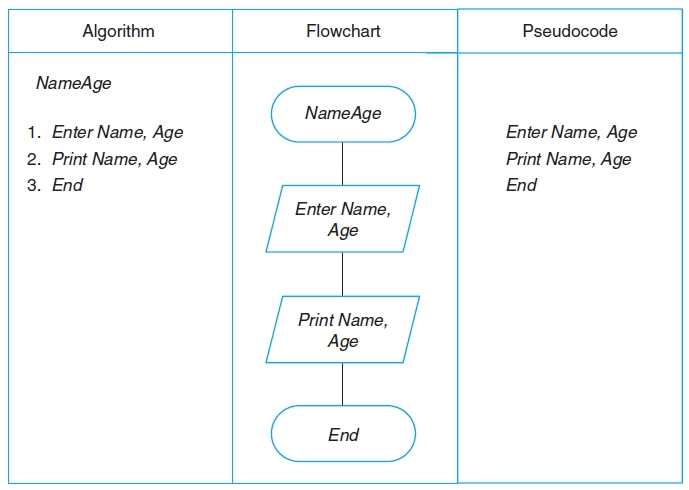
\includegraphics[width=10cm]{afp.jpg} \\
        {\tiny \sf Fonte: \cite[p. 93]{Sprankle2012} }
    \end{center}
   \end{figure}

   \section{\'{A}reas de Aplica\c{c}\~{a}o da Linguagem}
   Esta linguagem \'{e} utilizada e aplicada nas seguintes \'{a}reas: !!!!! As aqui mostradas s\~{a}o exemplos!!!

        \subsection{ Data Science}
        Fazer uma breve descri\c{c}\~{a}o. Pelo menos 3 par\'{a}grafos mencionando exemplos

        \subsection{ Orienta\c{c}\~{a}o a objetos}
        Fazer uma breve descri\c{c}\~{a}o. Pelo menos 3 par\'{a}grafos mencionando exemplos

        \subsection{ outras} 